%%%%%%%%%%%%%%%%%%%%%%%%%%%%%%%%%%%%%%%%%%%%%%%%%%%%%%%
%% Bachelor's & Master's Thesis Template             %%
%% Copyleft by Artur M. Brodzki & Piotr Woźniak      %%
%% Faculty of Electronics and Information Technology %%
%% Warsaw University of Technology, 2019-2020        %%
%%%%%%%%%%%%%%%%%%%%%%%%%%%%%%%%%%%%%%%%%%%%%%%%%%%%%%%

\documentclass[
    left=2.5cm,         % Sadly, generic margin parameter
    right=2.5cm,        % doesnt't work, as it is
    top=2.5cm,          % superseded by more specific
    bottom=3cm,         % left...bottom parameters.
    bindingoffset=6mm,  % Optional binding offset.
    nohyphenation=false % You may turn off hyphenation, if don't like.
]{eiti/eiti-thesis}

\langpol % Dla języka angielskiego mamy \langeng
\graphicspath{{img/}}             % Katalog z obrazkami.
\addbibresource{bibliografia.bib} % Plik .bib z bibliografią
\usepackage{float}
\usepackage{minted}

\begin{document}

%--------------------------------------
% Strona tytułowa
%--------------------------------------
\EngineerThesis % Dla pracy inżynierskiej mamy \EngineerThesis
\instytut{Informatyki i Automatyki Stosowanej}
\kierunek{Informatyka}
\specjalnosc{Inżynieria oprogramowania}
\title{
    Projekt i realizacja systemu do zgłaszania usterek w lokalach mieszkalnych.
}
\engtitle{ % Tytuł po angielsku do angielskiego streszczenia
    Design and implementation of a system for reporting faults in residential premises. 
}
\author{Krzysztof Fijałkowski}
\album{318652}
\promotor{dr Szymon Kijas}
\date{\the\year}
\maketitle

%--------------------------------------
% Streszczenie po polsku
%--------------------------------------
\clearpage % Zaczynamy od nieparzystej strony
\streszczenie Projekt ma na celu wytworzenie systemu wspierającego zarządzanie osiedlami mieszkaniowymi. W trakcie wytwarzania projektu zostały rozważone różne metody konteneryzacji oraz wdrażania projektu. Ostatecznie projekt został skonteneryzowany za pomocą Kubernetes'a, natomiast potok jego wdrożenia został wykonany za pomocą github actions. Została również wytworzona część monitoringu działania projektu za pomocą bazy elasticsearch, filebeat'u, logstash'a oraz kibana'y. Aplikacja API została wykonana za pomocą Pythona, natomiast interfejs użytkownika za pomocą Typescript'u, React'a oraz Vite. Użyta została również baza postgresql a komunikacja z nią odbywa się za pomocą ORM'u - SQLAlchemy. Zastosowano  również synchronizację między bazą postgresql a elasticsearch za pomocą pg\_sync.
\slowakluczowe konteneryzacja, Kubernetes, ELK, osiedla mieszkaniowe, zarządzanie

%--------------------------------------
% Streszczenie po angielsku
%--------------------------------------
\newpage
\abstract The project aims to create a system supporting the management of housing estates. During the project's development, various methods of containerization and project implementation were considered. Ultimately, the project was containerized using Kubernetes and its implementation pipeline was made using GitHub actions. A part of the project's operation monitoring was also created using the elasticsearch, filebeat, logstash and kibana databases. The API application was developed using Python, while the user interface was created using Typescript, React and Vite. A Postgresql database is also used and communication with it is carried out using an ORM - sqlalchemy. There is also the synchronization between the Postgresql database and elasticsearch using pg\_sync
\keywords containerization, Kubernetes, ELK, housing estates, management

%--------------------------------------
% Spis treści
%--------------------------------------
\cleardoublepage % Zaczynamy od nieparzystej strony
\tableofcontents

%--------------------------------------
% Rozdziały
%--------------------------------------
\cleardoublepage % Zaczynamy od nieparzystej strony
\pagestyle{headings}

\newpage % Rozdziały zaczynamy od nowej strony.
\section{Wprowadzenie}
\subsection{Cel pracy}
Celem niniejszej pracy było stworzenie systemu mającego na celu kompleksowe wsparcie administracji osiedla mieszkaniowego w najważniejszych obszarach działania, uwzględniając zarówno kwestie dotyczące obsługi mieszkańców, jak i zarządzania pracownikami spółdzielni. 
Jako jeden z wymienionych wyżej obszarów działania administracji osiedla zdefiniowano zagadnienie zgłaszania szkód, usterek i działań konserwacyjnych, zarządzanie zleceniami i rozliczeniem ich naprawy przy użyciu istniejących zasobów ludzkich. Przyjęto założenie, że projektowany system powinien więc pozwalać mieszkańcom na szybkie i wygodne zgłaszanie usterek do administracji osiedla mieszkaniowego, jak również  posiadać łatwo dostępne forum służące do informowania mieszkańców np. o awariach czy planowanych naprawach lub przekazywania ogólnej korespondencji dotyczącej budynku. 
Inną perspektywą, uwzględnioną w projektowanym rozwiązaniu, jest zarządzanie pracą osób wykonujących zlecenia dla spółdzielni, zaprojektowano rozwiązania umożliwiające przypisywanie pracowników do realizacji konkretnych zadań, jak i dodawanie nowych współpracujących osób i określanie ich ról. 
Przy projektowaniu systemu wzięto również pod uwagę taką jego budowę, aby  był przystosowany do obsługi wielu osiedli mieszkaniowych równocześnie. 
Nie mniej ważne było, aby aplikacja obsługiwała funkcjonalności istotne zarówno z perspektywy mieszkańca, jak i administratora osiedla, łącząc w jednym systemie całość zagadnień dotyczących budynku. 
System zaprojektowano w ten sposób, aby jego działanie było intuicyjne, przejrzyste i łatwe nawet dla niedoświadczonego użytkownika, uwzględniając różny stopień umiejętności informatycznych mieszkańców budynku.
Dla najefektywniejszej realizacji powyższych celów przyjęto, że oprogramowanie powinno być stworzone w środowisku skonteneryzowanym z hybrydową aplikacją internetową.
\subsection{Wprowadzenie do tematyki}
W dzisiejszym  społeczeństwie obserwujemy coraz większą potrzebę automatyzacji wszelkich procesów, możliwości użycia aplikacji w miejsce standardowej korespondencji, w tym również elastyczną możliwość komunikacji, niezależną od godzin pracy biur i urzędów. Zauważono, że jedną z takich dziedzin jest możliwość łatwego i szybkiego dokonywania różnych zgłoszeń przez mieszkańców budynku czy osiedla mieszkaniowego do administracji, uwzględniając drobne usterki, ale również poważniejsze awarie czy zgłoszenia o charakterze ogólnym związanym z zarządzaniem budynkiem. 

Projekt aplikacji powstał w celu zastąpienia osobistej wizyty w  administracji spółdzielni, w godzinach jej pracy i możliwość dokonania dowolnego zgłoszenia poprzez wygodne, nieskomplikowane i niezależne od pory dnia działanie w systemie. Jednocześnie, informacje i zawiadomienia przygotowane przez administrację dla mieszkańców będą dostępne nie tylko na tablicy ogłoszeń w wersji papierowej, ale także w sekcji ogłoszeń w aplikacji, tak aby każdy mógł się z nimi zapoznać w dogodnej formie. 

Projektowane rozwiązanie systemu zgłaszania wniosków i usterek będzie korzystne również dla osób z niepełnosprawnościami, zwiększając ich komfort i wygodę komunikacji, bez konieczności przemieszczania się do biura administracji. Uwzględniono również usługę dla osób niedowidzących, które za pomocą dedykowanego oprogramowania mogą odsłuchać treść aktualnych ogłoszeń administracyjnych.

Powyższe argumenty przedstawiają sprawność komunikacji mieszkańców z administracją w zakresie zgłaszania szkód, usterek czy awarii oraz zapoznawania się z aktualnościami. 

Warto zauważyć, że benefitem projektowanego systemu jest także połączenie dokonanych zgłoszeń z przypisaniem ich realizacji poszczególnym pracownikom, sprawność komunikacji wewnątrz administracji, a tym samym zwiększenie efektywności działań, skrócenie czasu reakcji i podniesienie sprawności działania obsługi konserwatorskiej.
\subsection{Analiza istniejących rozwiązań}
Na rynku mieszkaniowym istnieje wiele systemów zajmujących się podobną tematyką, aczkolwiek większość z nich zajmuje się obsługą spółdzielni jedynie od strony kadrowej, co jest również bardzo istotnym zagadnieniem, ale nie obejmującym obsługi mieszkańców. W odróżnieniu od dostępnych rozwiązań,  proponowane w tej pracy rozwiązanie koncentruje się  na obsłudze kontaktu mieszkaniec - administracja jak również zarządzaniu pracownikami realizującymi zlecenia. Poniżej przedstawione są niektóre z nich: 
\begin{itemize}
    \item Moja Spółdzielnia
    \item PROBIT
    \item System ADA
    \item emieszkaniec.pl
    \item imieszkaniec.pl
    \item mmsoft - lokalnet
    \item sacer
    \item mieszczanin.pl
\end{itemize}
\input{tex/02-analiza-wymagań}
\newpage 
\section{Metodologia wytwarzania}
W ramach tworzenia projektu  wytworzone zostały 3 repozytoria. Istnieją dwa główne powody ich rozdzielenia: każde repozytorium ma różniący się potok ciągłej integracji/ciągłego wdrażania, oraz każde repozytorium jest niezależnym modułem. Taki podział umożliwia również lepsze dbanie o porządek w poszczególnych modułach. Wszystkie repozytoria znajdują się na publicznym GitHub'ie, aby każdy miał do nich dostęp. 

Pierwszym z trzech repozytoriów jest repozytorium zawierające kod implementujący REST API napisany w Pythonie z użyciem FastApi oraz SQLAlchemy.

Drugim jest repozytorium zawierające kod implementujący interfejs użytkownika zaimplementowany z użyciem TypeScript'u, React-a oraz Tailwind'a.

Trzecim z nich jest repozytorium zawierające całą konfigurację wdrożenia, oraz detaliczną instrukcję, w jaki sposób to wdrożenie powinno zostać wykonane. Używane między innymi technologie to: Kubernetes, helm, ngnix.

Podczas tworzenia oprogramowania, z uwagi na  pracę jednoosobową, nie było potrzeby wykorzystywania metodologii podziału kolejnych zadań na odpowiednie branch'e, ponieważ nie było możliwości konfliktów ze względu na wspomnianą wyżej pracę jednoosobową. Kolejne funkcjonalności były dodawane w kodzie  na podstawie listy zadań istniejącej lokalnie. Z powodu ograniczonych możliwości technologicznych nie było również możliwości utworzenia testowego wdrożenia, więc istniał tylko jeden główny branch - main.

W celu wytworzenia oprogramowania korzystano z wielu narzędzi informatycznych, między innymi: 
\begin{itemize}
    \item Pycharm - w celu napisania aplikacji w Pythonie
    \item WebStorm - w celu napisania interfejsu użytkownika w TypeScript
    \item Docker Desktop - w celu testowania
    \item Hetzner - kupno i zarządzanie serwerem
    \item Tabby terminal - łączenie z serwerem
\end{itemize}
\newpage
\section{Definicja architektury}
\subsection{Schemat architektury}
Schemat architektury został wytworzony za pomocą metodologii C4, z użyciem narzędzia Icepanel. Narzędzie to jest przystosowane specjalnie do tworzenia diagramów w metodologii C4 i umożliwia bardzo czytelne wyświetlanie i modelowanie różnych architektur. Na diagramach system nazwany jest akronimem EMS (Estate Managment System) - System do zarządzania spółdzielniami.
\subsubsection{Kontekst}
Poniżej znajduje się pierwszy poziom diagramu C4 - kontekst, w tym przypadku nie jest on skomplikowany ze względu na brak integracji zewnętrznych systemów takich jak np. system do płatności.
\begin{figure}[H]
    \centering
    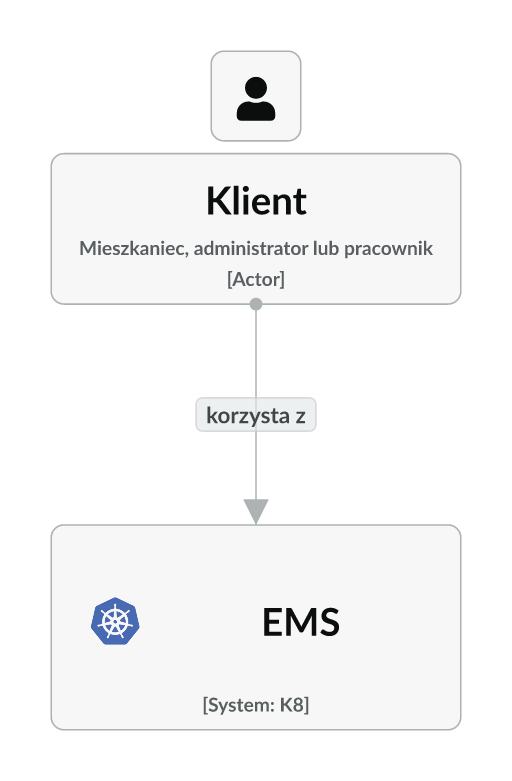
\includegraphics[width=0.5\linewidth]{img/Context_Diagram.png}
    \caption{Kontekst systemu}
    \label{fig:context-diag}
\end{figure}
\subsubsection{Kontener}
Kolejnym poziomem architektury C4 jest poziom kontenerów zaprezentowany poniżej. System został stworzony z użyciem Kubernetesa, tak więc całość jest opisana w klastrze Kubernetesowym z podziałem na poszczególne aplikacje, które zostaną opisane poniżej.
\begin{figure}[H]
    \centering
    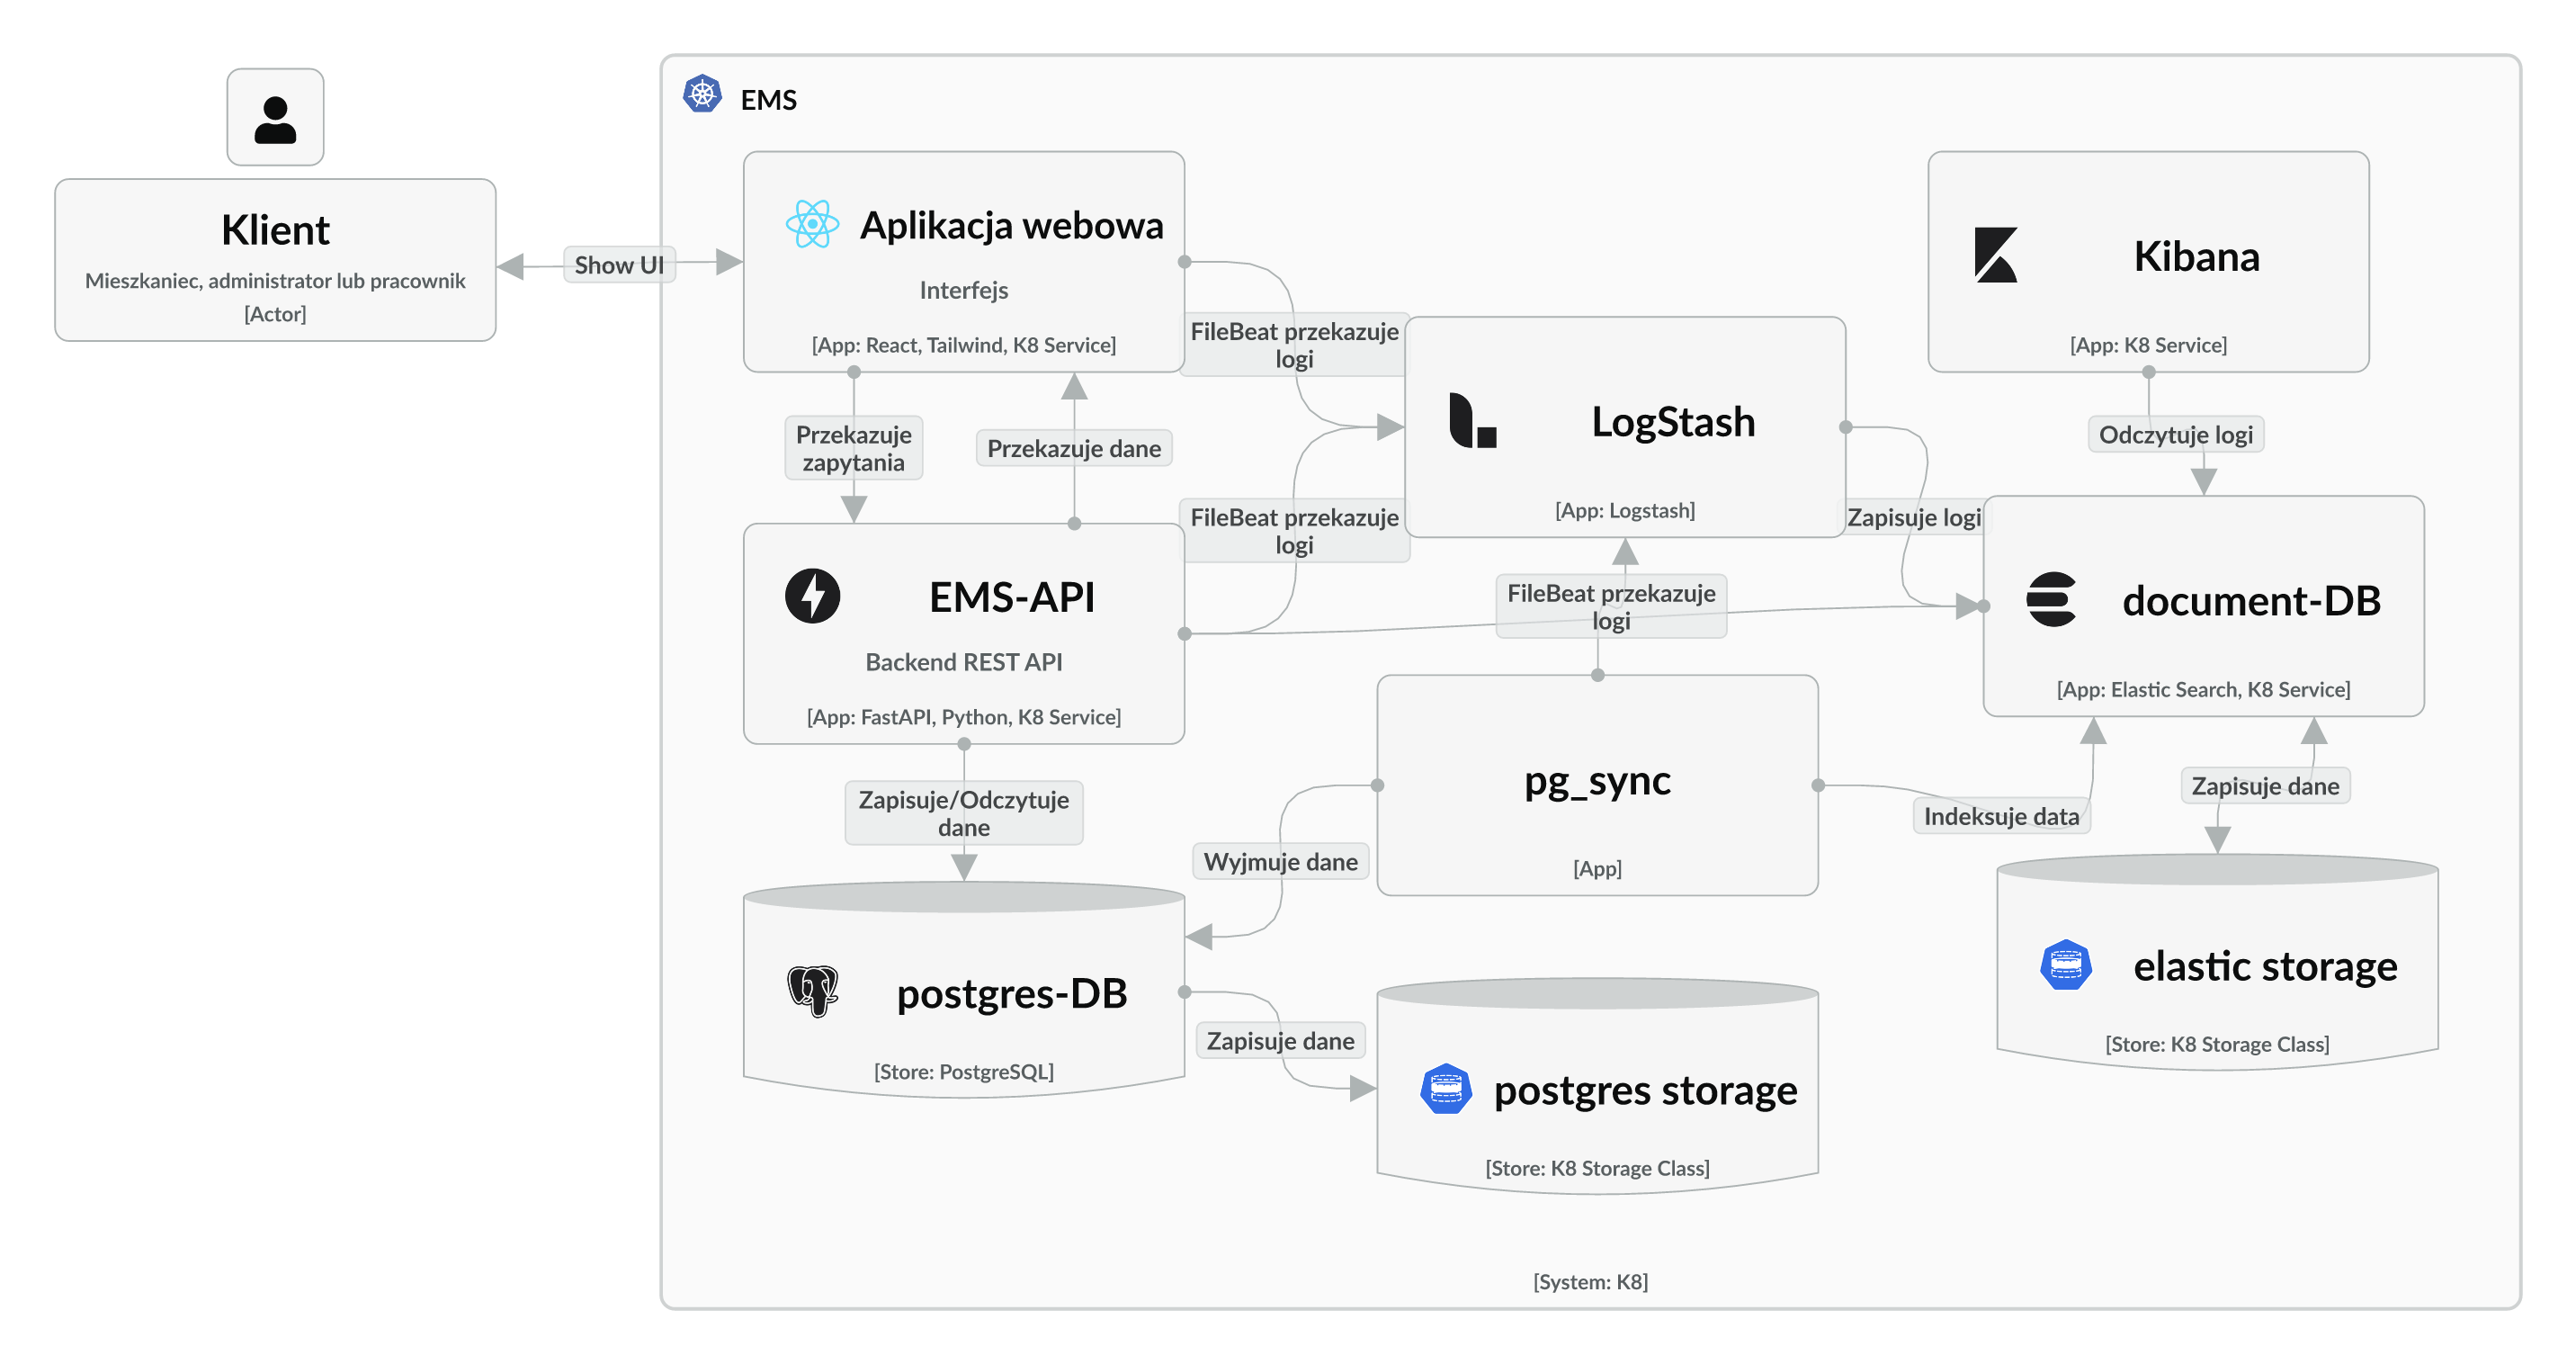
\includegraphics[width=1\linewidth]{img/Container_Diagram.png}
    \caption{Kontenery systemu}
    \label{fig:full-arch}
\end{figure}
Działanie systemu można podzielić na dwie części: część odpowiadającą za realizowanie funkcjonalności, oraz część odpowiadającą za monitorowanie systemu.

\subsubsection{Komponenty odpowiedzialne za realizowanie funkcjonalności}
\begin{itemize}
    \item \textbf{Aplikacja webowa} - jest to deployment Kubernetesowy znajdujący się w Kubernetesowym serwisie, deployment w Kubernetesie ma na celu zarządzanie między innymi na podstawie jakiego obrazu będą uruchamiane pody, oraz ich aktualną ilość kopii. Serwis jest abstrakcją sieciową mającą na celu umożliwienie komunikacji między podami za pomocą ich nazw. Aplikacja napisana została w TypeScript z użyciem React oraz Tailwind. Służy ona do wyświetlania interfejsu użytkownikowi. Interfejs jest dynamicznie renderowany u klienta (CSR). W tym module nie znajduje się żadna logika biznesowa, jest to tylko i wyłącznie warstwa reprezentacyjna komunikująca się z EMS-API.
    \item \textbf{EMS-API} - nazwa pochodzi od nazwy systemu EMS - System do zarządzania osiedlami. Jest to również Kubernetes'owy deployment w Kubernetes'owym serwisie. Jest to aplikacja napisana w Pythonie z użyciem FastApi wystawiający REST-API, z którego korzysta interfejs użytkownika. Moduł ten realizuje logikę biznesową. Komunikuje się on również z dwiema bazami danych: Postgres-DB oraz document-DB. Poniżej przedstawiono schemat reprezentujący znajdujące się w nim komponenty:
    \begin{figure}[H]
        \centering
        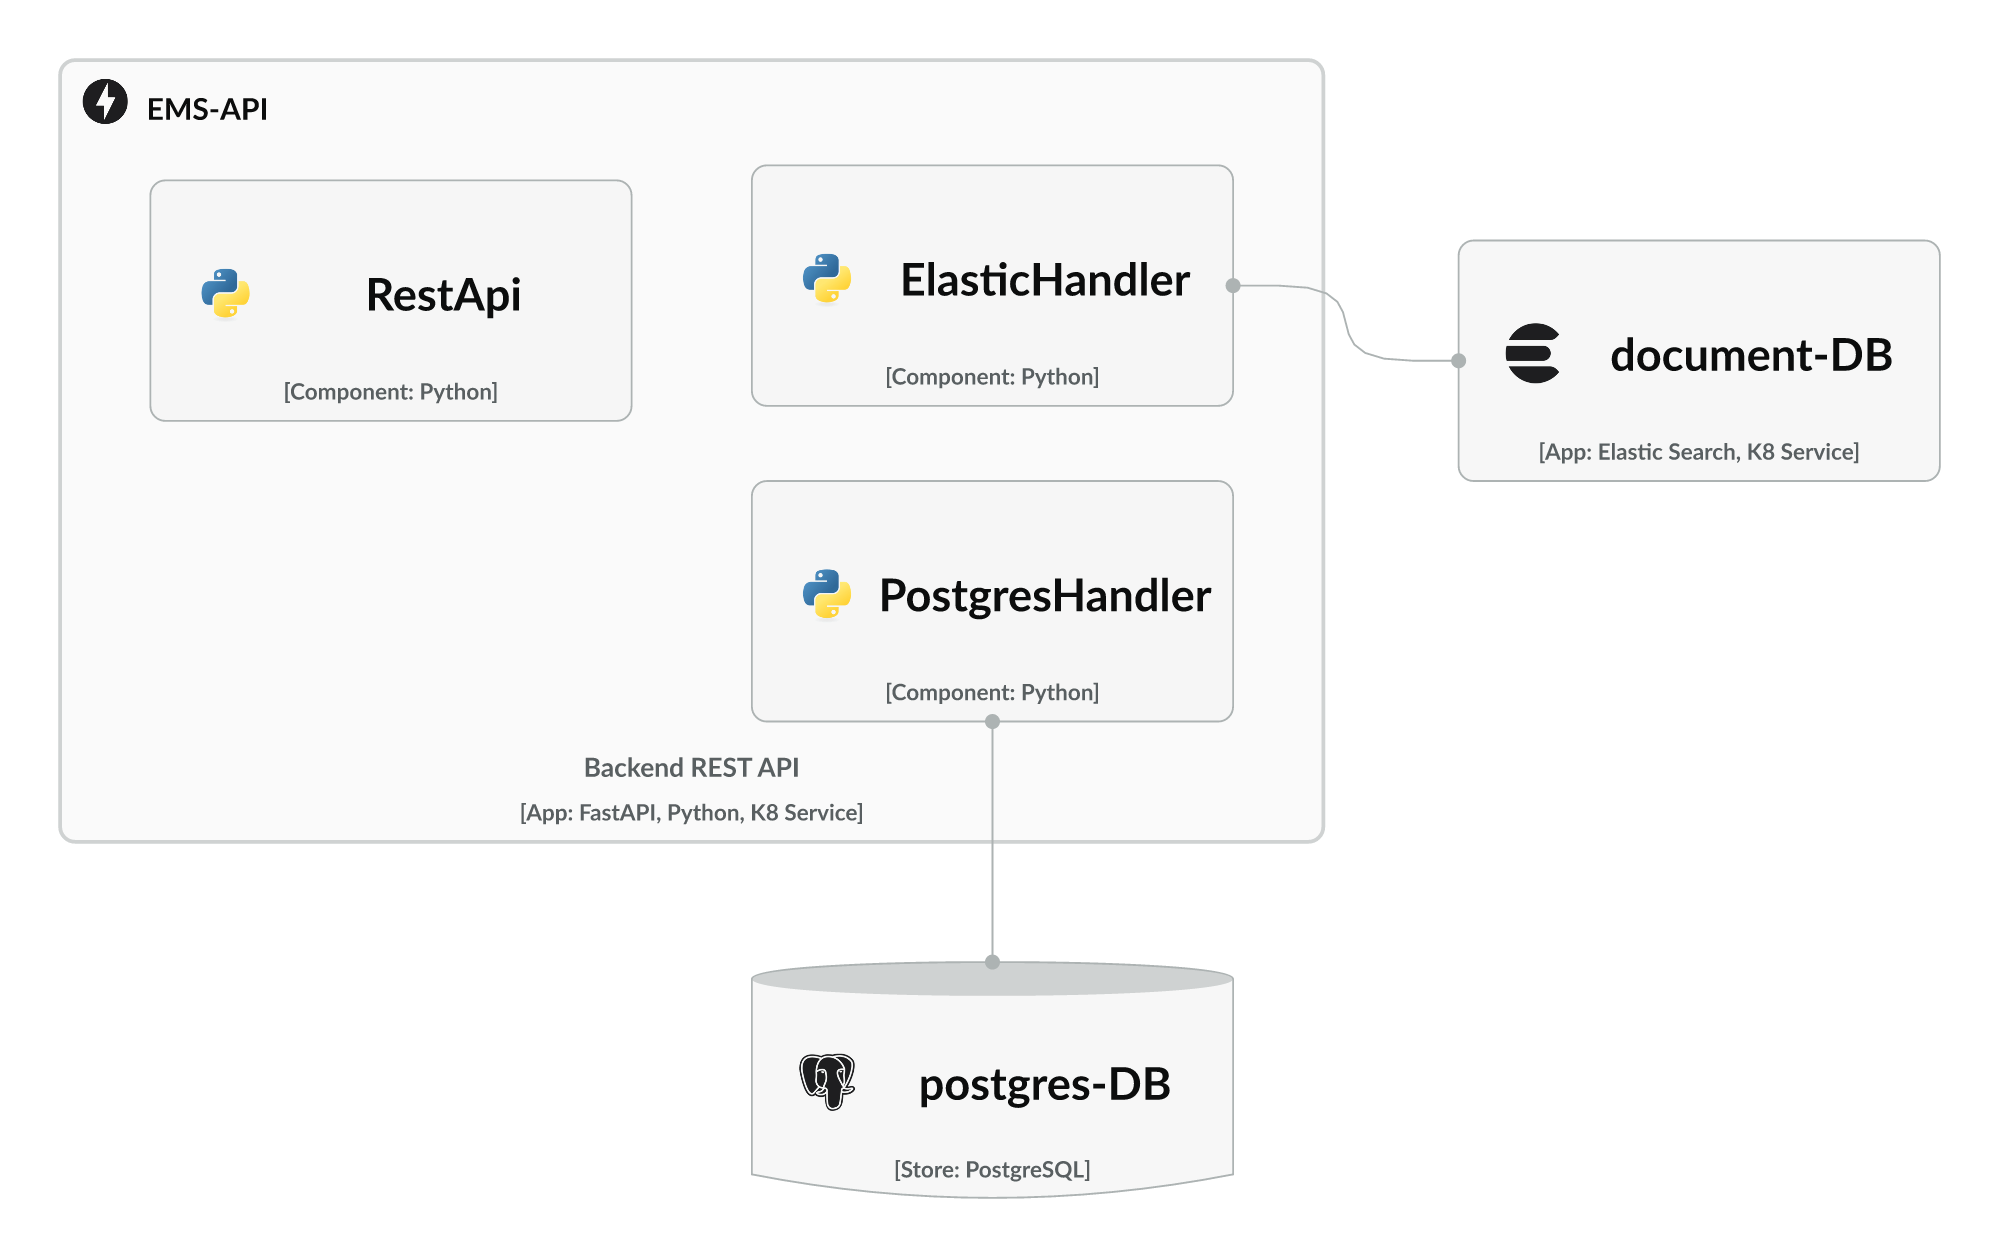
\includegraphics[width=0.75\linewidth]{img/EMS-API Component Diagram (Current).png}
        \caption{Diagram komponentów EMS-API}
        \label{fig:ems-api-components}
    \end{figure}
    \item \textbf{postgres-DB} - Baza relacyjna Postgres, w której zdefiniowane są relacje niezbędne do działania systemu. Jest to również Kubernetes'owy deployment w Kubernetes'owym serwisie.
    \item \textbf{postrges-storage} - Kubernetes'owy storage jest miejscem gdzie Postgres zapisuje dane, jest to niezbędny element, bez którego baza danych nie miała by miejsca na stabilne przetrzymywanie danych, używanie takiej abstrakcji umożliwia również relatywnie niskokosztową zmianę na inny typ storage-u.
    \item \textbf{document-DB} - Jest to baza NoSQL Elasticsearch w tym kontekście wykorzystywana do indeksowania pojedynczych elementów jak i do wyszukiwania elementów na podstawie ich fragmentów.
    \item \textbf{pg\_sync} - Jest to moduł open-source'owy służący do synchronizacji bazy relacyjnej - Postgres, oraz bazy noSQL - Elasticsearch. Moduł ten jest niezbędny ponieważ indeksuje on wybrane elementy w bazie dokumentowej, takimi przykładowymi elementami są np. treści postów. Dzięki temu wyszukiwanie postów na podstawie tekstu wpisanego przez użytkownika jest bardziej optymalne. Takie rozwiązanie odciąża również bazę Postgres - ponieważ wyszukiwanie na podstawie fragmentu tekstu nie jest w niej wykonywane. Moduł ten składa się z 2 elementów: aplikacji w języku Python oraz bazy Redis używanej jako kolejki, co zostało zobrazowane na poniższym diagramie:
    \begin{figure}[H]
        \centering
        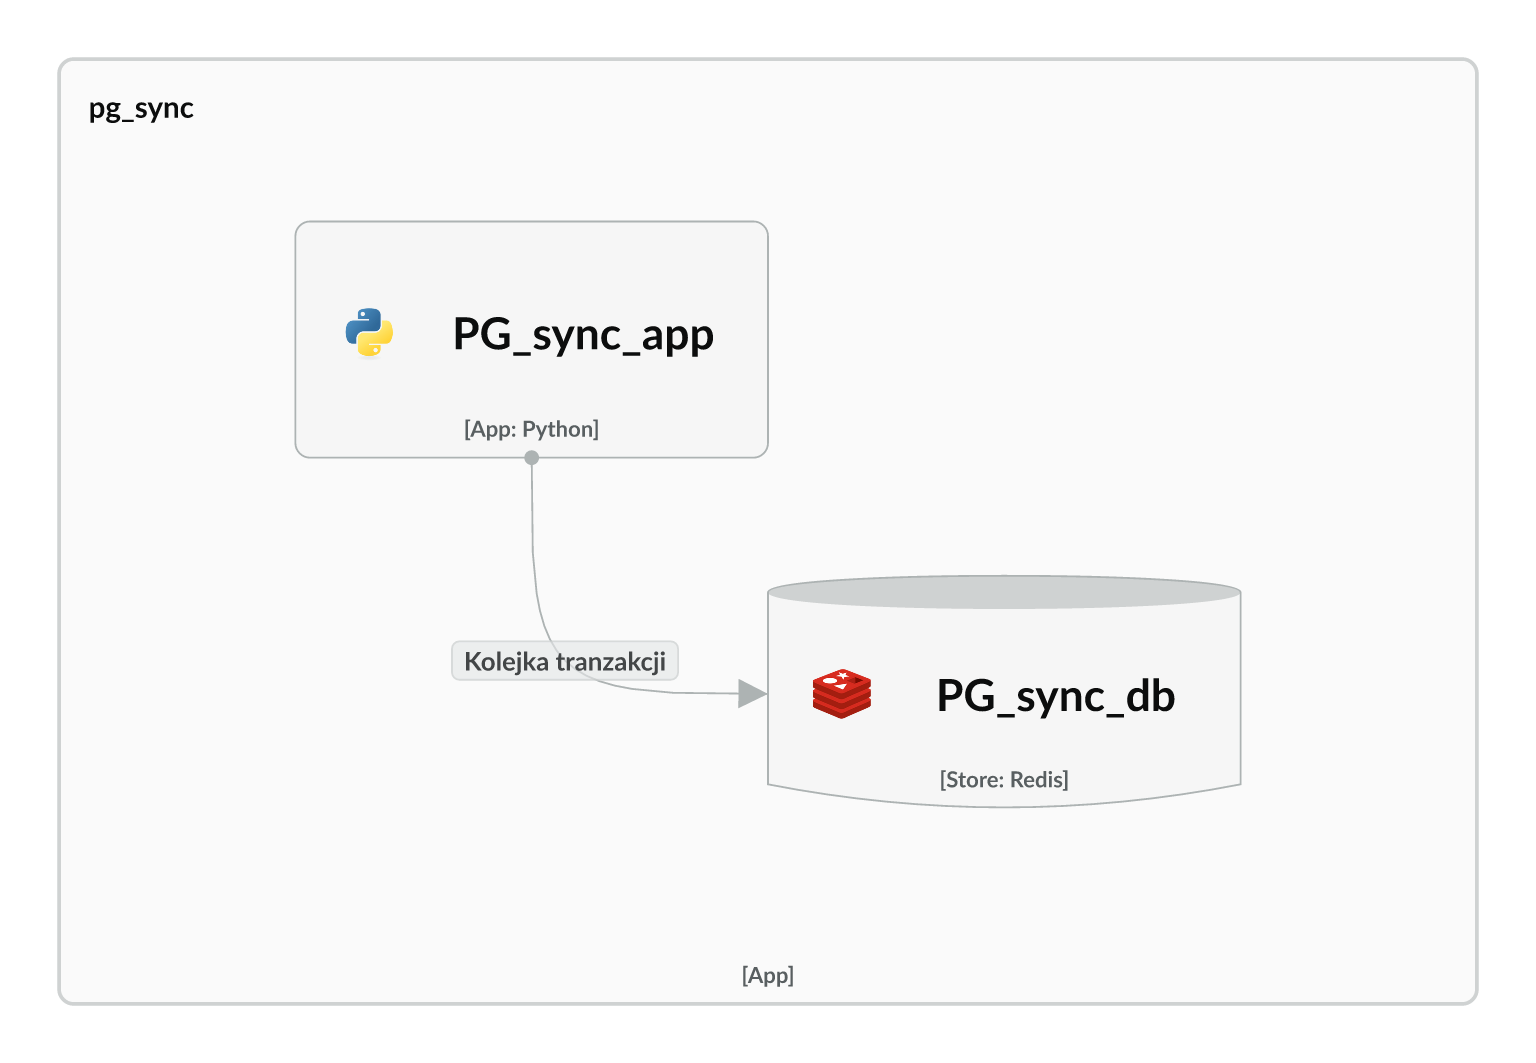
\includegraphics[width=0.75\linewidth]{img/pg_sync Component Diagram (Current).png}
        \caption{Diagram komponentów pg\_sync}
        \label{fig:pg_sync}
    \end{figure}
\end{itemize}
\subsubsection{Przepływ działania systemu  - perspektywa realizacji funkcjonalności}
W celu lepszej wizualizacji działania systemu, poniżej został dodany diagram przykładowego przepływu działania systemu, pokazujący proces dodania ogłoszenia przez użytkownika. Proces pokazuje tylko część systemu odpowiedzialną za działanie funkcjonalności.

\begin{figure}[H]
    \centering
    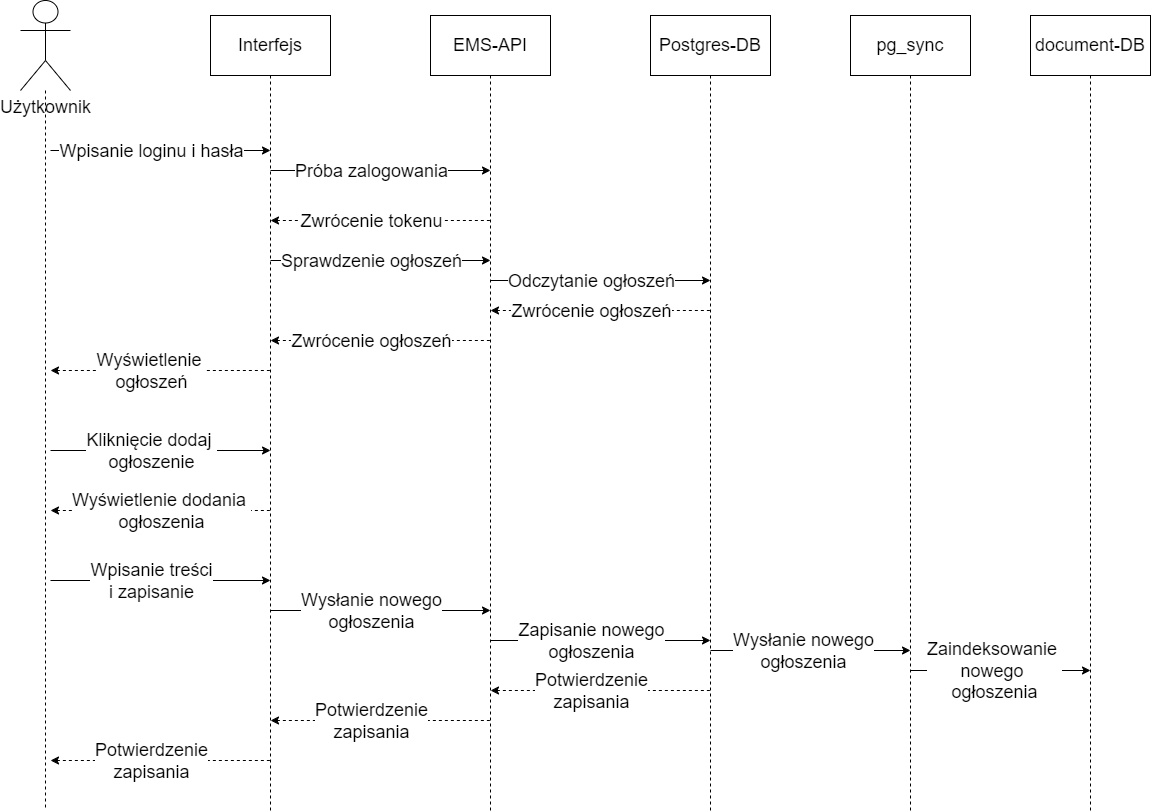
\includegraphics[width=1\linewidth]{img/sequence_diag_add_post.png}
    \caption{Diagram sekwencji dodania ogłoszenia}
    \label{fig:add_post_seq}
\end{figure}
\subsubsection{Komponenty odpowiedzialne za monitorowanie systemu}
\begin{itemize}
    \item \textbf{FileBeat} - Lekki open source'owy moduł stworzony przez firmę Elastic, służący do agregacji i przesyłania odnalezionych plików do skonfigurowanego miejsca, w tym przypadku jest to LogStash. Tak więc jest to komponent odnajdujący automatycznie logi z dodanych serwisów i przekazujący je do LogStash'a.
    \item \textbf{LogStash} - Open source'owe rozwiązanie stworzone przez firmę Elastic, służący do przyjmowania, przetwarzania oraz przekazywania logów do Elasticsearch.
    \item \textbf{document-DB} - Open source'owa baza NoSQL Elasticsearch firmy Elastic, w tym kontekście wykorzystywana jako miejsce zapisu i indeksowania logów.
    \item \textbf{Kibana} - Open source'owe rozwiązanie firmy Elastic stworzone w celu wizualizacji danych znajdujących się w tym przypadku w Elasticsearch, posiada również między innymi możliwość tworzenia dashboard'ów zwiększających potencjał wizualizacji danych, tutaj - logów.
\end{itemize}


\subsection{Decyzje architektoniczne}
\subsubsection{Sposób konteneryzacji, dlaczego Kubernetes?}

Pod uwagę zostało wziętych wiele możliwości konteneryzacji systemów, takich jak:
\begin{itemize}
    \item \textbf{Docker Compose} - Rozwiązanie to umożliwia uruchamianie aplikacji złożonych z wielu kontenerów Docker'owych, nie ma ono wbudowanych wielu możliwości dostępnych w Kubernetes'ie, takich jak równoważenie obciążenia (ang: load balancing). Jest dobre do lokalnego testowania aplikacji, lub wdrażania małych rozwiązań.
    \item \textbf{Docker swarm} - Jest to rozwiązanie wbudowane w silnik Docker'a umożliwiające zarządzanie tworzonymi kontenerami i dostarczające podstawowe funkcjonalności przydatne przy wdrożeniu, takie jak równoważenie obciążenia. Jest ono o wiele mniej popularne od Kubernetes'a i posiada o wiele mniejsze wsparcie. Na podstawie pracy \cite{KubernetesVSDockerSwarm} można wywnioskować, że Kubernetes jest bardziej skomplikowanym narzędziem, posiadającym więcej funkcjonalności, podczas gdy Docker swarm jest rozwiązaniem prostszym i jednocześnie bardziej optymalnym.
    \item \textbf{Podman} - Jest to dobre rozwiązanie do zarządzania pojedynczymi podami na jednej maszynie, nie jest ono dobre do wdrażania dużych aplikacji.
\end{itemize}
Wszystkie te rozwiązania mają swoje plusy i minusy, i po dokładnej ich analizie został wybrany Kubernetes, jako rozwiązanie dostarczające najwięcej możliwości rozwoju, skalowalności i oferujące największe wsparcie społeczności informatycznej.
\subsubsection{Technologia monitorowania działania systemu}
Monitorowanie działania danego systemu jest niezbędnym aspektem, który należy rozważyć, przy prostych aplikacjach skonteneryzowanych na bazie Dockera/Docker-compose często wystarczającym może być obserwowanie logów poszczególnych kontenerów. 

W Kubernetes'ie problem jednak jest większy ze względu na, między innymi, liczbę replik danych aplikacji. Dobrym przykładem jest EMS-API, jest to aplikacja mająca 3 repliki, należy więc wziąć pod uwagę, że w sytuacji wystąpienia błędu, osoba nadzorująca działanie systemu powinna zalogować się na serwer, a następnie wykonać kontrolę  kolejnych logów w każdym podzie, co nie jest ani wygodne ani optymalne.

Często spotykanym rozwiązaniem jest dodatkowy system do monitorowania działania aplikacji, wiele osób korzysta w tym przypadku  z tzw. "ELK stack", będącego połączeniem rozwiązań open-source'owych dostarczonych przez firmę Elastic, w celu monitorowania np. logów. Wymienione rozwiązanie zostało wykorzystane  w projektowanych systemie, z uwagi  na jego popularność i wsparcie społeczeństwa programistycznego. Mając na względzie rozwój aplikacji, jest ono bardzo wygodne, ponieważ dodanie kolejnego elementu systemu nie wymaga praktycznie żadnego nakładu pracy z perspektywy systemu monitoringu, aby ten element również był monitorowany.
\subsubsection{Dobór typu bazy danych}
Do realizacji projektu, będącego celem niniejszej pracy,  wymagana jest baza relacyjna, rynek informatyczny oferuje szeroki wybór dostępnych baz tego rodzaju. Na podstawie analizy artykułu \cite{fi16100382} możemy wywnioskować, że baza Postgres jest o wiele wydajniejsza od bazy MySQL z perspektywy odczytu danych z bazy jak i ich zapisu. Baza Postgres jest odpowiednią bazą do realizacji tego projektu. Aby odciążyć tę bazę można również zutylizować bazę Elasticsearch i indeksować w niej wybrane elemenenty z bazy relacyjnej.
\subsubsection{Sposób synchronizacji Postgres'a z Elasticsearch}
Aby móc użyć 2 baz,  potrzebny jest sposób ich niezawodnej synchronizacji, na rynk dostępnych jest wiele takich  rozwiązań, np: Logstash JDBC input plugin proponowany przez Elastic jako rozwiązanie do synchronizacji bazy Postgres oraz Elasticsearch. Po przeanalizowaniu tego rozwiązania zostało ono odrzucone ze względu na skomplikowaną konfigurację. Rozwiązaniem, które ostatecznie wybranno,  jest pg\_sync open source,  umożliwiające synchronizację bazy Postgres z bazą elastic przy użyciu minimalnej konfiguracji. Pg\_sync złożony jest z aplikacji w Pythonie i kolejki z użyciem Redis'a, tak więc jest to rozwiązanie wygodne do skonteneryzowania, co jest kolejnym atutem.
\subsubsection{Sposób komunikacji z bazami danych}
Istnieje wiele sposobów utworzenia tabel w bazie relacyjnej i komunikacji z nią z perspektywy Pythona. Jedną z możliwości stanowi pisanie plików w SQL, mające na celu tworzenie odpowiednich tabel i funkcji ułatwiających komunikację, ale istnieją też inne dobre rozwiązania. Jednym z takich rozwiązań jest użycie ORM-u: mapowanie obiektowo-relacyjne, polegające na odwzorowaniu relacji z bazy w sposób obiektowy w kodzie. Aby to zrealizować można skorzystać z Pythonowej paczki SQLAlchemy, dzięki czemu nie istnieją pliki w sql tylko i wyłącznie w Pythonie, a tym samym istnieje mniej rozproszonych źródeł oprogramowania, co wspiera zarządzanie wersją i zmniejsza potencjał popełnienia błędów. Dzięki użyciu ORM-a jesteśmy również w stanie napisać testy jednostkowe do metod wykonywanych na bazie. Jednocześnie, zmiana typu bazy z perspektywy kodu aplikacji jest wtedy bardzo prosta - zmieniamy typ silnika ORM-u. Należy rozważyć również  negatywne aspekty tego podejścia, omówione w artykule \cite{ImpactOfORM}, na podstawie którego można wywnioskować, że ORM ma duży wpływ na wydajność zapytań kierowanych do bazy, ale jednocześnie daje on dużą swobodę programistom implementującym użycie bazy z użyciem ORM-a zamiast zapytań SQL.
\newpage
\section{Implementacja EMS-API}
Implementację możemy podzielić na dwa główne moduły - implementację aplikacji w Pythonie - EMS-API, która zostanie omówiona w tym rozdziale, oraz implementację interfejsu użytkownika w TypeScript, która będzie omówiona w kolejnym.

\subsection{Podział kodu}
Implementacja systemu EMS-API może zostać podzielona na implementację API, połączenia do Postgres oraz połączenia do Elasticsearch.

\textbf{Paczki:}
\begin{itemize}
    \item app - paczka z kodem implementującym API
    \item database - paczka z kodem implementującym podłączenie do bazy Postgres
    \item elastic\_utils - paczka z kodem implementującym podłączenie do Elasticsearch
    \item package\_utils - paczka z częściami wspólnymi np. implementacją logger'a
\end{itemize}


\subsection{Implementacja API}
\subsubsection{Podział kodu w API}
\begin{itemize}
    \item models - paczka z kodem reprezentującym modele. Modele są to definicje formatu danych przyjmowanych i zwracanych przez API
    \item routers - implementacja router'ów
    \item utils - paczka z częściami wspólnymi kodu
    \item main.py - główny plik API łączący wszystkie router'y
\end{itemize}
\subsubsection{Implementacja main.py}
API zostało zaimplementowane z pomocą biblioteki FastApi, która umożliwia wygodne definiowanie kolejnych endpoint'ów oraz podział logiczny kodu na kolejne pliki z zdefiniowanymi endpoint'ami. W głównym pliku znajduje się dodanie router'ów:
\begin{minted}{python}
    app = FastAPI()
    
    app.include_router(posts_router.router)
    app.include_router(security_router.router)
    app.include_router(estates_router.router)
    ...
\end{minted}
\subsubsection{Implementacja przykładowego router-a}
Każdy z routerów jest odpowiednio zdefiniowaną grupą end-pointów, w których możemy określić między innymi czy wymagane jest, aby użytkownik był zalogowany w momencie próby pozyskania danych z endpoint'u: poprzez użycie "dependencies". Poniżej przykład konfiguracji router'a z prefix-em requests do obsługi zgłoszeń:
\begin{minted}{python}
    router = APIRouter(
        prefix="/requests",
        tags=["requests"],
        responses={404: {"description": "Not found"}},
        dependencies=[Depends(get_current_active_user)]
    )
\end{minted}

W ramach danego router'a jesteśmy w stanie zdefiniować wiele endpoint'ów, w których definiujemy poza parametrami wejściowymi, w jakim formacie mają być zwrócone dane używając: response\_model. Poniżej przykład endpoint'u do odczytania konkretnego zgłoszenia: 
\begin{minted}{python}
    @router.get("/{request_id}", response_model=Optional[RequestInfo])
    async def get_request_( request_id: str,
                            current_user: Annotated[Users, 
                            Depends(get_current_active_user)],
                            db: Session = Depends(get_db)):
        return get_request(db, request_id, current_user.id)
\end{minted}
Jak można zauważyć, używany jest w nim response\_model: RequestInfo. Wszystkie takie modele zdefiniowane są w  folderze models.
\subsubsection{Implementacja przykładowego modelu}
Poniżej znajduje się implementacja przykładowego modelu, są to klasy, których reprezentacje są przekazywane do i z API.
\begin{minted}{python}
    from pydantic import BaseModel

    class RequestInput(BaseModel):
        title: str
        description: str
    
    class RequestInfo(RequestInput):
        id: str
        author_id: str | None
        title: str
        description: str
        department: str | None
        status: str
        start_time: datetime.datetime
        end_time: datetime.datetime | None
        assignee_id: str | None
        visibility: str
\end{minted}
\subsection{Implementacja połączenia z bazą Postgres}
Do obsługi bazy danych wykorzystany został ORM - SQLAlchemy, umożliwiający reprezentację relacji jako obiekty w kodzie.
\subsubsection{Podział kodu}
\begin{itemize}
    \item declarations - paczka ze zdefiniowanymi relacjami
    \item utils.py - plik z częściami wspólnymi kodu
\end{itemize}
\subsection{Implementacja użycia bazy Postgres}
W celu połączenia zdefiniowano url oraz tworzona jest sesja, która jest przekazywana do funkcji wykonujących operacje na bazie.
\begin{minted}{python}
    url = URL.create(
        drivername="postgresql+pg8000",
        username=POSTGRESQL_USERNAME,
        password=POSTGRESQL_PASSWORD,
        host=POSTGRESQL_HOST,
        port=POSTGRESQL_PORT,
        database=DATABASE_NAME
    )
    SessionLocal = sessionmaker(autocommit=False, autoflush=False,
                                bind=SqlEngine().engine)
\end{minted}
\subsubsection{Sposób reprezentacji relacji}
Każda relacja ma odwzorowanie w obiekcie. Relacje zaimplementowane zostały na podstawie modelu stworzonego w narzędziu dbdiagram:
\begin{figure}[H]
    \centering
    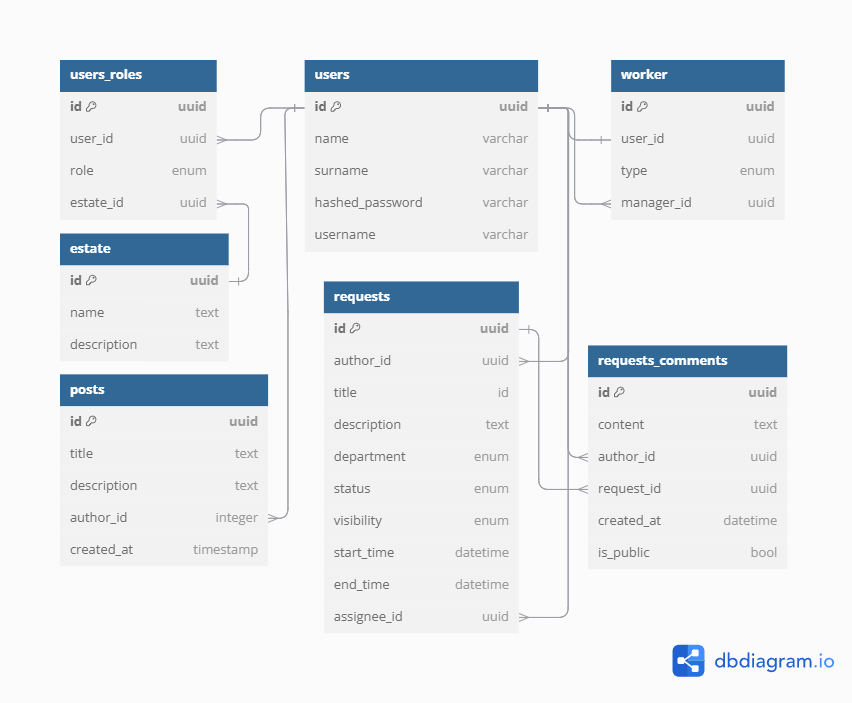
\includegraphics[width=1\linewidth]{img/ER_model.png}
    \caption{Model relacji}
    \label{fig:data model}
\end{figure}
Poniżej znajduje się reprezentacja relacji Requests (zgłoszenia) w kodzie Pythona z użyciem SQLAlchemy:
\begin{minted}{python}
    class Requests(Base):
        __tablename__ = "requests"

        id: Mapped[str] = mapped_column(primary_key=True, default=uuid.uuid4)
        author_id: Mapped[str] = mapped_column(ForeignKey(Users.id))
        title: Mapped[str] = mapped_column(String)
        description: Mapped[str] = mapped_column(String)
        department: Mapped[Enum] = mapped_column(Enum(Department),
                                                 nullable=True)
        status: Mapped[Enum] = mapped_column(Enum(Status), 
                                             default=Status.NEW)
        visibility: Mapped[Enum] = mapped_column(Enum(Visibility), 
                                                 default=Visibility.PRIVATE)
        start_time: Mapped[datetime.datetime] = mapped_column(DateTime)
        end_time: Mapped[datetime.datetime] = mapped_column(DateTime, 
                                                            nullable=True)
        assignee_id: Mapped[str] = mapped_column(ForeignKey(Users.id),
                                                 nullable=True)
\end{minted}

SQLAlchemy udostępnia wiele możliwości, takich jak reprezentowanie obiektów typem Enum zdefiniowanym w Pythonie, czy obiektami datetime. Daje to możliwość wygodniejszego użycia i analizowania działania bazy danych.

\subsubsection{Sposób korzystania z obiektów SQLAlchemy}
Jesteśmy w stanie zdefiniować funkcje używające konkretnych obiektów w celu np. wydobycia z nich danych, SQLAlchemy dostarcza możliwość nie pisania SQL-a tylko korzystania z zaimplementowanej biblioteki do budowania zapytań do bazy. Poniżej znajduje się przykład takiej funkcji zwracającej konkretne zgłoszenie:

\begin{minted}{python}
    def get_request(session, request_id: str, user_id: str) -> Requests | None:
        user_estate = get_user_estate_id(session, user_id)
        return (session.query(Requests)
                .select_from(Requests)
                .join(UsersRoles, 
                      UsersRoles.user_id == Requests.author_id)
                .filter(Requests.id == request_id,
                        UsersRoles.estate_id == user_estate)
                .first())
\end{minted}

\subsection{Implementacja użycia Elasticsearch'a}
\subsubsection{Struktura kodu}
\begin{itemize}
    \item queries.py - plik zawierający funkcje przeszukujące bazę
    \item utils.py - plik definiujący klienta
\end{itemize}
\subsubsection{Stworzenie klienta oraz wyszukanie informacji w bazie}
W celu połączenia z bazą Elasticsearch wykorzystana została biblioteka Elasticsearch, za pomocą której można utworzyć klienta oraz przeszukać bazę. Do przeszukiwania fragmentów tekstów w poszczególnych indeksach została wytworzona generyczna funkcja get\_ids\_for\_index\_containing. Oba te elementy można zaobserwować poniżej.
\begin{minted}{python}
    # utils.py file
    es_client = (
    Elasticsearch("http://elasticsearch-master.elk.svc.cluster.local:9200",
                  basic_auth="elastic",
                  verify_certs=False)
                )

    # queries.py file
    def get_index_for_id_containing(index: str, phrase: str) -> List[str]:
    """
    Get the id field of the hit containing the phrase in given index
    :param index: index name (eg. posts)
    :param phrase: phrase to look for
    :return: List of post ids
    """
        resp = es_client.search(index=index, 
                                query={"match": {"description": phrase}})
        return [x["_source"]["id"] for x in resp["hits"]["hits"]]
\end{minted}
\subsection{Konfiguracja pg\_sync}
Aby odpowiednie relacje były indeksowane w Elasticsearch należy dobrze skonfigurować pg\_sync. W ramach takiej konfiguracji poza plikiem przekazującym informacje o adresach i hasłach do baz, niezbędny jest również plik definiujący, które relacje powinny być indeksowane. Poniżej znajduje się fragment takiego pliku konfiguracyjnego wskazującego pg\_sync, aby indeksował trzy pola relacji posts: id, title oraz description.
\begin{minted}{json}
[
    {
        "database": "estate_management",
        "index": "posts",
        "nodes": {
            "table": "posts",
            "columns": [
                "id",
                "title",
                "description"
            ]
        }
    }
]
\end{minted}



\newpage
\section{Implementacja interfejsu użytkownika}
Interfejs użytkownika został zaimplementowany za pomocą języka typescript przy użyciu  biblioteki react pozwalającej na budowanie aplikacji internetowych. Użyto również framework-u css-owego tailwind umożliwiającego wygodne dostosowanie graficzne elementów strony. Do budowania strony użyto narzędzia Vite umożliwiającego zarówno budowanie wersji produkcyjnych jak i deweloperskich (odświeżających się w momencie zmiany kodu) w wygodny sposób.
\subsection{Podział kodu}
\begin{itemize}
    \item \textbf{assets} - pliki graficzne
    \item \textbf{components} - implementacje poszczególnych podstron
    \item \textbf{App.tsx} - główny komponent aplikacji zwracający Router aplikacji
    \item \textbf{index.css} - definicja użycia styli tailwind'a
    \item \textbf{main.tsx} - główny plik interfejsu zwracający główny komponent - App
    \item \textbf{router.tsx} - definicja routera aplikacji
    \item \textbf{types.tsx} - definicja typów użytych w aplikacji
\end{itemize}
\subsection{Implementacja komponentów}
W ramach interfejsu użytkownika zostały utworzone następujące podfoldery implementujące różne komponenty:
\begin{itemize}
    \item \textbf{estateAdmin} - komponenty odpowiedzialne za panel administratora
    \item \textbf{layout} - komponenty związane z całą stroną, np: Header
    \item \textbf{posts} - komponenty związane z ogłoszeniami
    \item \textbf{register}\_login - komponenty związane z logowaniem oraz rejestracją
    \item \textbf{requests} - komponenty związane ze zgłoszeniami
    \item \textbf{userPage} - strona użytkownika
    \item \textbf{utils} - wspólne części używane w wielu miejscach, np przycisk
\end{itemize}

Omówienie jednego z tych folderów umożliwi zrozumienie implementacji wszystkich, takim przykładowym folderów jest "requests", w którym znajdują się następujące pliki:
\begin{itemize}
    \item \textbf{comments} - komponenty związane z komentarzami pod danym zgłoszeniem
    \item \textbf{single} - komponenty związane z wyświetlaniem pojedynczego zgłoszenia
    \item \textbf{addRequest.tsx} - komponent zawierający formularz dodania pojedynczego zgłoszenia
    \item \textbf{fetches.ts} - plik zawierający wszystkie zapytania do API związane ze zgłoszeniami
    \item \textbf{RequestCard.tsx} - komponent wyświetlający pojedyncze zapytanie w formie kafelka
    \item \textbf{ViewRequests.tsx} - komponent wyświetlający wszystkie dostępne zapytania w formie kafelków
\end{itemize}
Większość komponentów składa się z podobnych elementów. Poniżej przedstawione są elementy komponentu requests/single/ViewRequest.
Pierwszym powtarzającym się elementem jest \textbf{zdefiniowanie zmiennych}
\begin{minted}{js}
export function ViewRequest() {
    const { requestId } = useParams<{ requestId: string }>();
    const [request, setRequest] = useState<RequestType>();
\end{minted}
Kolejnym jest \textbf{załadowanie danych}:
\begin{minted}{js}
useEffect(() => {
    getRequest(requestId!)
        .then((data) => setRequest(data))
        .catch((_) => {
            toastHelper.error("Wystąpił błąd :(. Spróbuj jeszcze raz");
        });
}, []);
\end{minted}
Załadowanie danych odbywa się za pomocą funkcji zdefiniowanej w pliku \textbf{request/fetches.ts}:
\begin{minted}{js}
export const getRequest = async (id: string): Promise<RequestType> => {
    const response = await fetch(`${API_ADDR}requests/${id}`, 
                                getSecureRequestOptions);
    if (!response.ok) {
        throw new Error("HTTP error " + response.status);
    }
    return await response.json();
}
\end{minted}
Typ używany powyżej \textbf{RequestType} zdefiniowany jest w pliku types.ts, który jest wspólny dla całej aplikacji. Poniżej znajduje się jego fragment definiujący RequestType:
\begin{minted}{js}
// Requests
export type RequestType = {
    id: string;
    author_id: string;
    title: string;
    description: string;
    department: string;
    status: string;
    start_time: string;
    end_time: string;
    assignee_id: string;
    visibility: string;
}
\end{minted}
Następnym elementem jest \textbf{zwrócenie odpowiednich komponentów}:
\begin{minted}{html}
return (
    <div>
        {isEmploye ? (
            <EditableView request={request} authorName={authorName} />
        ) : (
            <UserView request={request} authorName={authorName} />
        )}
        <div>
            <AllComments request_id={request.id} />
            <AddComment request_id={request.id} />
        </div>
    </div>
);
\end{minted}
Powyżej widzimy, że w zależności od typu użytkownika wyświetlane są poszczególne komponenty, zamieszczono przykład implementacji jednego z tych funkcji:
\begin{minted}{html}
function EditableView(props: { request: RequestType, authorName: string }) {
    return <div 
    className="p-12 grid grid-cols-1 md:grid-cols-2 gap-16 justify-center">
        <RequestInfo request={props.request} authorName={props.authorName}/>
        <RequestEdit request={props.request}/>
    </div>;
}
\end{minted}

Style pojedynczych komponentów często są poprawiane za pomocą przekazywania do zmiennej className odpowiednich atrybutów.

\newpage
\section{Dokładna implementacja wybranych funkcjonalności}
\subsection{Logowanie}
W implementacji logowania pomocnym był poradnik \cite{FastapiAuthLearn}.
Poniżej znajduje się diagram przepływu logowania, pokazują szczegółowo jego proces:

\begin{figure}[H]
    \centering
    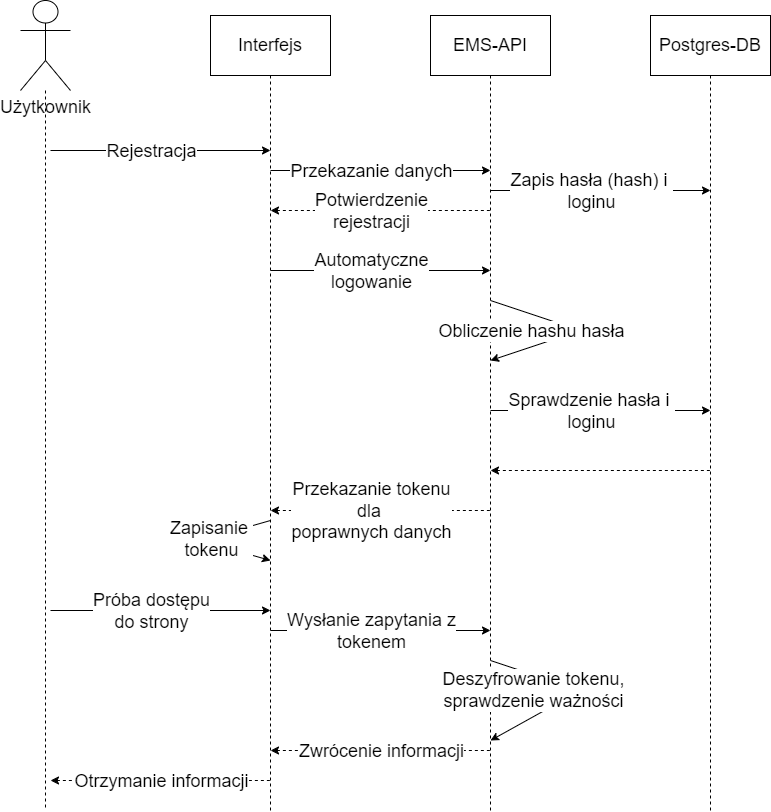
\includegraphics[width=0.75\linewidth]{img/sequence_login.png}
    \caption{Diagram przepływu logowania}
    \label{fig:seq-diag-login}
\end{figure}
Podczas logowania hasło użytkownika jest hash'owane oraz zapisywane w bazie za pomocą biblioteki passlib korzystającej z funkcji bcrypt. Podczas weryfikacji jest używana metoda verify.
\begin{minted}{python}
def verify_password(plain_password, hashed_password):
    return pwd_context.verify(plain_password, hashed_password)
\end{minted}

Gdy hasło użytkownika jest poprawne, tworzony jest token JWT. Token jest szyfrowany za pomocą klucza oraz algorytmu "HS256". Jest on następnie przekazywany klientowi oraz zapisany w local storage. Utworzenie tokenu o ważności 15 minut:
\begin{minted}{python}
def create_access_token(data: dict, expires_delta: timedelta | None = None):
    to_encode = data.copy()
    if expires_delta:
        expire = datetime.now(timezone.utc) + expires_delta
    else:
        expire = datetime.now(timezone.utc) + timedelta(minutes=15)
    to_encode.update({"exp": expire})
    encoded_jwt = jwt.encode(to_encode, SECRET_KEY, algorithm=ALGORITHM)
    return encoded_jwt
\end{minted}
Zapisanie go w local storage:
\begin{minted}{js}
    localStorage.setItem("accessToken", data.access_token);
\end{minted}
Przekazanie wraz z kolejnymi zapytaniami w nagłówku zapytania w celu weryfikacji:
\begin{minted}{js}
    method: "GET",
    headers: {
        "Content-Type": "application/json",
        "Authorization": `Bearer ${localStorage.getItem("accessToken")}`,
    }
\end{minted}
Przekazany token jest sprawdzany, na podstawie tokenu weryfikowany jest użytkownik oraz ważność tokenu.
\begin{minted}{python}
...
try:
    payload = jwt.decode(token, SECRET_KEY, algorithms=[ALGORITHM])
    username: str = payload.get("sub")
    if username is None:
        raise credentials_exception
    token_data = TokenData(username=username)
except InvalidTokenError:
    raise credentials_exception
...
\end{minted}
Po weryfikacji tokenu oraz użytkownika API zwraca konkretne informacje.
\newpage
\section{Wdrożenie}
\subsection{Konteneryzacja poszczególnych modułów}
Konteneryzacja ma na celu możliwość wdrożenia poszczególnych aplikacji w systemie Kubernetes'owym, oraz możliwość testowania produktów w emulowanym środowisku produkcyjnym. Dzięki niej produkt nasz jest bardziej niezależny od środowiska, w którym jest uruchamiany i nie ma on wpływu na to środowisko. Aby skonteneryzować pewne serwisy można skorzystać z Docker'a, poprzez napisanie odpowiednich dockerfile'i. Skonteneryzowane zostały w ten sposób natępujace elementy:
\begin{itemize}
    \item EMS-API
    \item Interfejs użytkownika
    \item pg\_sync
\end{itemize}
Poniżej znajduje się przykładowy dockerfile serwisu EMS-API. Składa się on z:
\begin{itemize}
    \item Definicji wykorzystywanego obrazu bazowego - w tym przypadku jest to obraz posiadający Pythona 3.12
    \item Instalację potrzebnych paczek
    \item Skopiowanie kodu źródłowego
    \item Wystawienie odpowiedniego portu
    \item Uruchomienie aplikacji
\end{itemize}
\begin{minted}{docker}
FROM python:3.12

WORKDIR /product

COPY ./requirements.txt /code/requirements.txt

RUN pip install --no-cache-dir --upgrade -r /code/requirements.txt

COPY ./code /product/code

EXPOSE 8080

CMD ["fastapi", "run", "code/app/main.py", "--port", "8080"]
\end{minted}
Kolejne komponenty są skonteneryzowane w podobny sposób.

\subsection{Potok}
\begin{figure}[H]
    \centering
    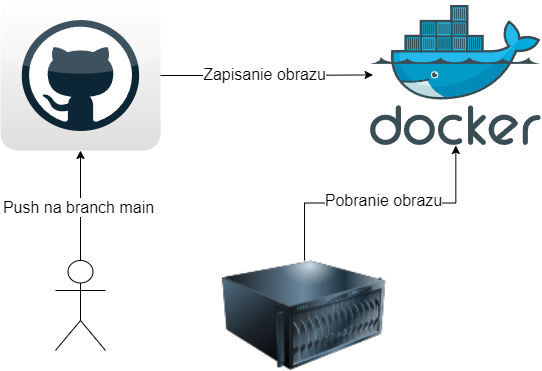
\includegraphics[width=0.7\linewidth]{img/inz_deploy.png}
    \caption{Potok wdrożenia}
    \label{fig:deploy-pipeline}
\end{figure}
Potok wdrożenia jest taki sam dla repozytoriów EMS-API oraz interfejsu użytkownika. Można podzielić go na kolejne etapy, pierwszym z nich jest push'owanie nowej wersji kodu na główny branch repozytorium przez programistę, następnie za pomocą github actions są wykonywane kolejne operacje: testowanie w przypadku EMS-API, następnie zbudowanie obrazu oraz wgranie go do publicznego repozytorium docker-hub. Kolejnym ważnym etapem jest wgranie nowej wersji na produkcję.

\subsubsection{Github actions}
Jest to narzędzie, które nie wymaga dodatkowej konfiguracji czy wdrożenia, jak na przykład Jenkins, ponieważ jest ono wbudowane w github'a. Dzięki temu, w sytuacji, gdy repozytorium jest ulokowane na github'ie, dodanie do niego konkretnych github actions wymaga tylko pojedynczego pliku konfiguracyjnego. W ramach jednego pliku konfiguracyjnego można zdefiniować wiele kroków koniecznych do wykonania. W przykładowym potoku wdrożenia aplikacji EMS-API są 3 takie kroki:
\begin{itemize}
    \item Testowanie
    \item Budowanie obrazu oraz wysłanie go do docker-repository
    \item Wdrożenie produktu na produkcję
\end{itemize}
Każdy z job'ów ma kolejne steps, które są wykonywane w kolejności od góry do dołu. Job'y mogą być wykonywane równolegle, aczkolwiek można definiować między nimi zależności, w tym potoku zależności te wyglądają następująco.
\begin{figure}[H]
    \centering
    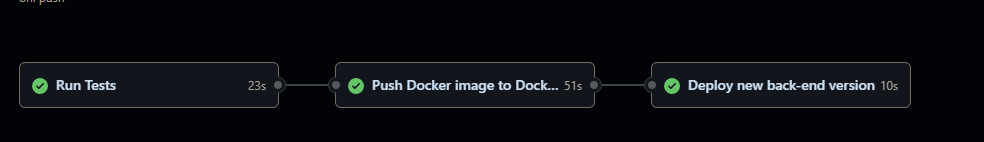
\includegraphics[width=0.75\linewidth]{img/potok-joby.png}
    \caption{Diagram zależności job-ów w potoku}
    \label{fig:jobs-dep}
\end{figure}

Poniżej znajduje się fragment odpowiedzialny za testowanie nowo dodanego kodu - pierwszy job w całym potoku. Ten job wykonuje się zazwyczaj w około 20 sekund.
\begin{minted}{yaml}
run_tests:
name: Run Tests
runs-on: ubuntu-latest
steps:
  - name: Check out the repo
    uses: actions/checkout@v4

  - name: Set up Python
    uses: actions/setup-python@v4
    with:
      python-version: '3.x'
  
  - name: Install dependencies
    run: pip install -r requirements.txt
  
  - name: Run tests
    run: python -m pytest
\end{minted}
Kolejnym etapem jest zbudowanie i wysłanie nowego obrazu do publicznego repozytorium docker'owego, etap ten zajmuje zazwyczaj poniżej minuty. Poniżej znajdują się trzy wybrane fragmenty. W pierwszym możemy zaobserwować, że job ten zależny jest od poprawnego wykonania job'u run\_tests. W kolejnym widać, że z perspektywy actions do docker hub logujemy się za pomocą hasła i loginu umieszczonego w sekretach repozytorium na github. W ostatnim wypychamy gotowy obraz do stworzonego wcześniej repozytorium gambolkf/inz-back.
\begin{minted}{yaml}
name: Push Docker image to Docker Hub
runs-on: ubuntu-latest
needs: run_tests
(...)
  - name: Log in to Docker Hub
    uses: docker/login-action@f4ef78c080cd8ba55a85445d5b36e214a81df20a
    with:
      username: ${{ secrets.DOCKER_USERNAME }}
      password: ${{ secrets.DOCKER_PASSWORD }}
(...)

  - name: Generate artifact attestation
    uses: actions/attest-build-provenance@v1
    with:
      subject-name: docker.io/gambolkf/inz-back
      subject-digest: ${{ steps.push.outputs.digest }}
      push-to-registry: true
\end{minted}
Po wykonaniu tego etapu możemy zaobserwować nowy obraz na docker-hub o nazwie gambolkf/inz-back z tagiem main.

\begin{figure}[H]
    \centering
    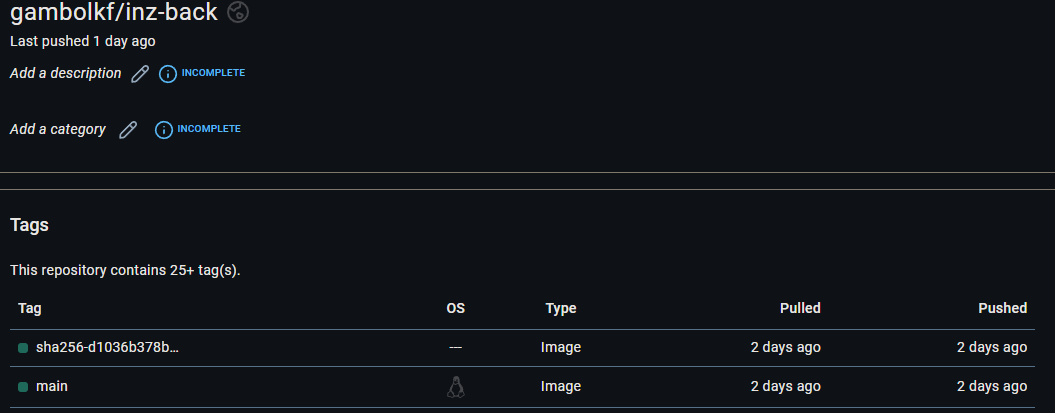
\includegraphics[width=0.75\linewidth]{img/docker-hub-screen.png}
    \caption{Docker-hub obrazy}
    \label{fig:docker0hub-img}
\end{figure}


Ostatnim etapem jest wgranie nowej wersji aplikacji na serwer produkcyjny, odbywa się to za pomocą wywołania komendy Kubernetes'owej- po ssh. Hasło do serwera znajduje się w sekretach github-a.
\begin{minted}{yaml}
deploy_image:
    name: Deploy new back-end version
    runs-on: ubuntu-latest
    needs: push_to_registry
    permissions:
      packages: write
      contents: read
      attestations: write
      id-token: write
    steps:
      - name: Install sshpass
        run: sudo apt-get update && sudo apt-get install -y sshpass

      - name: Restart Deployment on Remote Server
        env:
          SSH_PASSWORD: ${{ secrets.SSH_PASSWORD }}
        run: |
          sshpass -p "$SSH_PASSWORD" ssh -o StrictHostKeyChecking=no kfijalk@49.13.73.66 \
          "minikube kubectl -- rollout restart deployment/fastapi-app -n back"
\end{minted}



\subsection{Stworzenie  odpowiednich abstrakcji Kubernetes'owych}
Aby użyć dockerfile'i w Kubernetes'ie potrzebne jest stworzenie odpowiednich plików konfiguracyjnych. 
\subsubsection{Aplikacje EMS-API, pg\_sync, interfejs użytkownika}
Poniżej znajduje się przykład pliku konfiguracyjnego odpowiadającego za deployment EMS-API. Deployment jest to typ abstrakcji Kubernetes'owej odpowiedzialnej za wdrożenie i zarządzanie pod'ami, ich wersją obrazu, ich ilością, i wieloma innymi elementami. W tym konkretnym Deployment'cie definiujemy jako wersję obrazu obraz: gambolkf/inz-back:main który został wgrany poprzez potok na publiczne repozytorium docker-a. Została również ustawiona flaga imagePullPolicy, dzięki której w momencie restartu tego Deploymentu obraz jest ładowany na nowo. Dzięki takiej konfiguracji za pomocą komendy: `kubectl -- rollout restart deployment/fastapi-app -n back` zostanie wgrana nowa wersja tego deploymentu. Został również wystawiony port 8080 aby był dostęp do API.
\begin{minted}{yaml}
apiVersion: apps/v1
kind: Deployment
metadata:
  name: fastapi-app
  namespace: back
spec:
  replicas: 3
  selector:
    matchLabels:
      app: fastapi-app
  template:
    metadata:
      labels:
        app: fastapi-app
    spec:
      containers:
        - name: fastapi-app
          image: gambolkf/inz-back:main
          imagePullPolicy: Always
          ports:
            - containerPort: 8080
\end{minted}
Kolejną niezbędną abstrakcją jest Kubernetes'owy service. Abstrakcja ta umożliwia komunikację z daną grupą pod'ów za pomocą nazwy serwisu, zamiast np. poszczególnych adresów ip podów. Istnieją różne  typy serwisów, gdzie dla EMS-API najlepszym typem jest NodePort, ponieważ dzięki niemu możemy zdefiniować jaki port jest wystawiony poza sieć Kubernetes'a i po tym porcie komunikować się z danym serwisem z sieci zewnętrznej. Powiązanie między deploymentem a servicem realizowane jest za pomocą sekcji selector, w której zdefiniowane zostało app na tą samą wartość co w deploymencie.
\begin{minted}{yaml}
apiVersion: v1
kind: Service
metadata:
  name: fastapi-app-service
  namespace: back
spec:
  type: NodePort
  ports:
    - port: 80
      targetPort: 8080
      nodePort: 30001
  selector:
    app: fastapi-app
\end{minted}

Dla aplikacji pg\_sync oraz interfejsu użytkownika zarówno deployment jak i service został zdefiniowany analogicznie. Aby pg\_sync mógł działać poprawnie, koniecznie było uruchomienie bazy redis, zostało wykonane to z pomocą helm, następującą komendą:
\begin{minted}{bash}
helm install my-redis bitnami/redis --version 20.3.0
\end{minted}

\subsubsection{Wdrożenie bazy danych Postgres}
Etap ten wykonany jest zgodnie z poradnikiem \cite{DigitalOtionPostgresToK8s}
W celu wdrożenia bazy danych Postgres został również zdefiniowany deployment oraz service. Poza tymi abstrakcjami zostały również wykorzystane: config-map w celu zdefiniowania nazwy bazy, użytkownika oraz hasła. Persistance-Volume zastosowano w celu rezerwacji miejsca na serwerze. Wdrożenie wykonano za pomocą poniższych materiałów:
\begin{minted}{yaml}
apiVersion: v1
kind: PersistentVolume
metadata:
  name: postgres-volume
  labels:
    type: local
    app: postgres
spec:
  storageClassName: manual
  capacity:
    storage: 10Gi
  accessModes:
    - ReadWriteMany
  hostPath:
    path: /data/postgresql
\end{minted}
Zastosowano również persistance-volume claim, które umożliwia korzystanie z danego persistance-volume pod-om
\begin{minted}{yaml}
apiVersion: v1
kind: PersistentVolumeClaim
metadata:
  name: postgres-volume-claim
  labels:
    app: postgres
spec:
  storageClassName: manual
  accessModes:
    - ReadWriteMany
  resources:
    requests:
      storage: 10Gi
\end{minted}

Poza abstrakcjami Kubernetes'owymi, w celu zapewnienia  współpracy bazy z pg\_sync,  wymagane było ustawienie jej dwóch parametrów: wal\_level na logical oraz max\_replication\_slots na więcej niż 1. Wykonane to zostało za pomocą następujących komend wykonanych wewnątrz bazy:
\begin{minted}{bash}
ALTER SYSTEM SET wal_level = logical; ALTER SYSTEM SET max_replication_slots = 5;
\end{minted}
\subsubsection{ELK}
W wykonaniu tego etapu pomocnym był poradnik \cite{ELKTutorial}.
W celu wdrożenia aplikacji monitoringu nazywanych ELK stack, wykorzystany został menadżer pakietów Kubernetes'owych: helm. Zostały pobrane odpowiednie pakiety: elasticsearch, kibana, filebeat, logstash. W większości została przeprowadzona mała edycji plików konfiguracyjnych values.yaml. Dla przykładu, w przypadku pliku konfiguracyjnego elasticsearch edytowane zostały wymagania JVM-a w celu pomniejszenia zapotrzebowania RAM-u. Po edycji, każda z tych aplikacji została zainstalowana za pomocą komendy:
\begin{minted}{bash}
helm install <nazwa aplikacji> <ścieżka do folderu z paczką instalacyjną>
\end{minted}

\subsection{Środowisko produkcyjne}
Jako środowisko produkcyjne wybrany  został serwer na platformie Hetzner. Była to najlepsza forma symulacji środowiska produkcyjnego w najbardziej ekonomicznym rozwiązaniu. Na tym serwerze uruchomiony został klaster Kubernetes'owy za pomocą minikube-a. Jest to narzędzie tworzące mają instancję Kubernetes'a z jednym node-em. Ze uwagi  na tę konkretną konfigurację, zaistniała konieczność dodania narzędzia Ngnix do przekazywania komunikacji na serwer do node-a Kubernetes'owego. Poniżej znajduje się fragment konfiguracji przekazujący komunikację na odpowiedni port node-u.
\begin{minted}{bash}
server {
    listen 80;
    server_name 49.13.73.66;

    location / {
        proxy_pass http://192.168.49.2:30000;
        ...
\end{minted}

Pod adres IP serwera została podpięta również domena. W tym celu wykupiona została domena krzysztof-fij-inz.pl. Jednocześnie na platformie clodflare został zdefiniowany DNS: 
\begin{figure}[H]
    \centering
    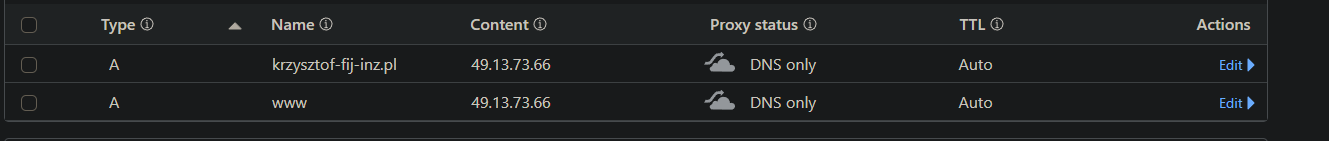
\includegraphics[width=1\linewidth]{img/dns_cloudflare.png}
    \caption{DNS}
    \label{fig:DNS-label}
\end{figure}
Dzięki temu dostęp do serwisu realizowany jest poprzez odwiedzenie domeny krzysztof-fij-inz.pl.

\newpage
\section{Testowanie}
W ramach projektu zostały wykonane 2 typy testów: jednostkowe oraz manualne. Aplikacja EMS-API była testowana z użyciem testów jednostkowych, natomiast interfejs użytkownika z użyciem testów manualnych. Istnieją narzędzia umożliwiające testowanie interfejsów internetowych, takie jak: selenium web driver, czy Playwrite, aczkolwiek w tak wczesnej fazie projektu, przy częstych zmianach interfejsu, dogodniejsze jest zastosowanie testów manualnych. Czas i zasoby poświęcone na implementację poprawnych testów interfejsu mogłyby zająć o wiele dłużej, niż czas poświęcony na regularne testowanie manualne. Testy manualne interfejsu użytkownika były wykonywane zgodnie z instrukcją interfejsu użytkownika.
\subsection{Implementacja testów jednostkowych}
Testy jednostkowe zostały wykonane za pomocą biblioteki pytest-sqlalchemy-mock. Biblioteka ta mockuje połączenie do bazy danych w SQLAlchemy używając technologii pytest oraz fixtures. Dzięki temu działaniu, w momencie pisania testu jednostkowego, do funkcji przekazywany jest argument "mocked\_session", dzięki któremu wykonujemy funkcje na zmockowanej bazie. Relacje i dane początkowe w bazie zdefiniowane są za pomocą słownika, którego fragment znajduje się poniżej.
\begin{minted}{python}
mock_db = {
  "estate": [
      {
          "id": 1,
          "name": "Test Estate",
          "description": "Test Estate Description"
      }...
  ],
  "users": [
      { ...
\end{minted}
Należy zauważyć, że rozwiązanie to posiada pewne ograniczenia, mianowicie, aby mockować bazę, biblioteka ta wykorzystuje sql-light, który nie wspiera wszystkich typów danych, wspieranych natomiast w bazach Postgres. Takim przykładem jest typ UUID, który używany jest w projekcie do dodawania nowych obiektów w bazie. Poniżej znajduje się przykładowy test.
\begin{minted}{python}
def test_get_post(mocked_session):
    post = get_post(mocked_session, "1")
    assert post.title == "Test Post"
    assert post.description == "Test Post Description"
    assert post.author_id == "1"
\end{minted}

\newpage
\section{Monitorowanie działania systemu}
Monitorowanie działania systemu realizowane było  za pomocą zbierania i analizy logów. W celu ułatwienia analizy,  został utworzony panel do obserwacji. Panel taki można wykonać za pomocą narzędzia - Kibana. Narzędzie to ma wiele możliwości, takich jak przeszukiwanie istniejących logów czy tworzenie paneli. Przeszukania  aktualnych logów dokonujemy przy użyciu widoku Discover, w którym możliwe jest  wyszukanie logów na podstawie nazw kontenera z którego pochodzą, na podstawie frazy w nich zawartej, ich daty, czy wielu innych parametrów:
\begin{figure}[H]
    \centering
    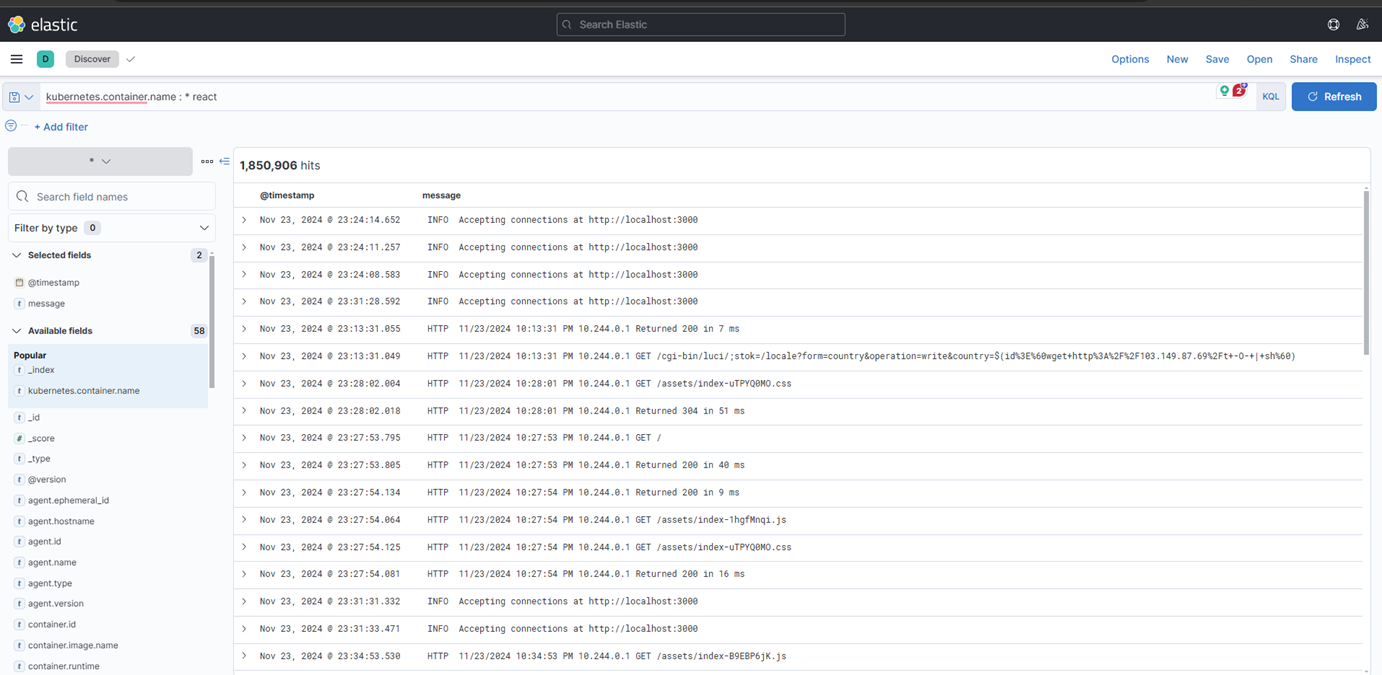
\includegraphics[width=1\linewidth]{logs_view.png}
    \caption{Wyświetlenie logów w kibanie}
    \label{fig:kibana-logs}
\end{figure}

Dzięki wbudowanym w narzędzie Kibana modułu do analiz, możemy wytworzyć analizy całości logów. Na analizie przedstawionej poniżej,  w pierwszej sekcji od góry znajdują się aktualne logi, następnie poniżej, licząc od lewej: liczba wszystkich logów, liczba logów informujących o error'ach oraz stosunek tych ostatnich względem sumy wszystkich. W ostatnim rzędzie prezentowane są  wykresy obrazujące: które kontenery pokazują najwięcej logów związanych z error'ami oraz jak zapis logów w czasie. Dla dokładniejszej wizualizacji, można dowolnie dobrać przedział czasowy do prezentacji danych.
\begin{figure}[H]
    \centering
    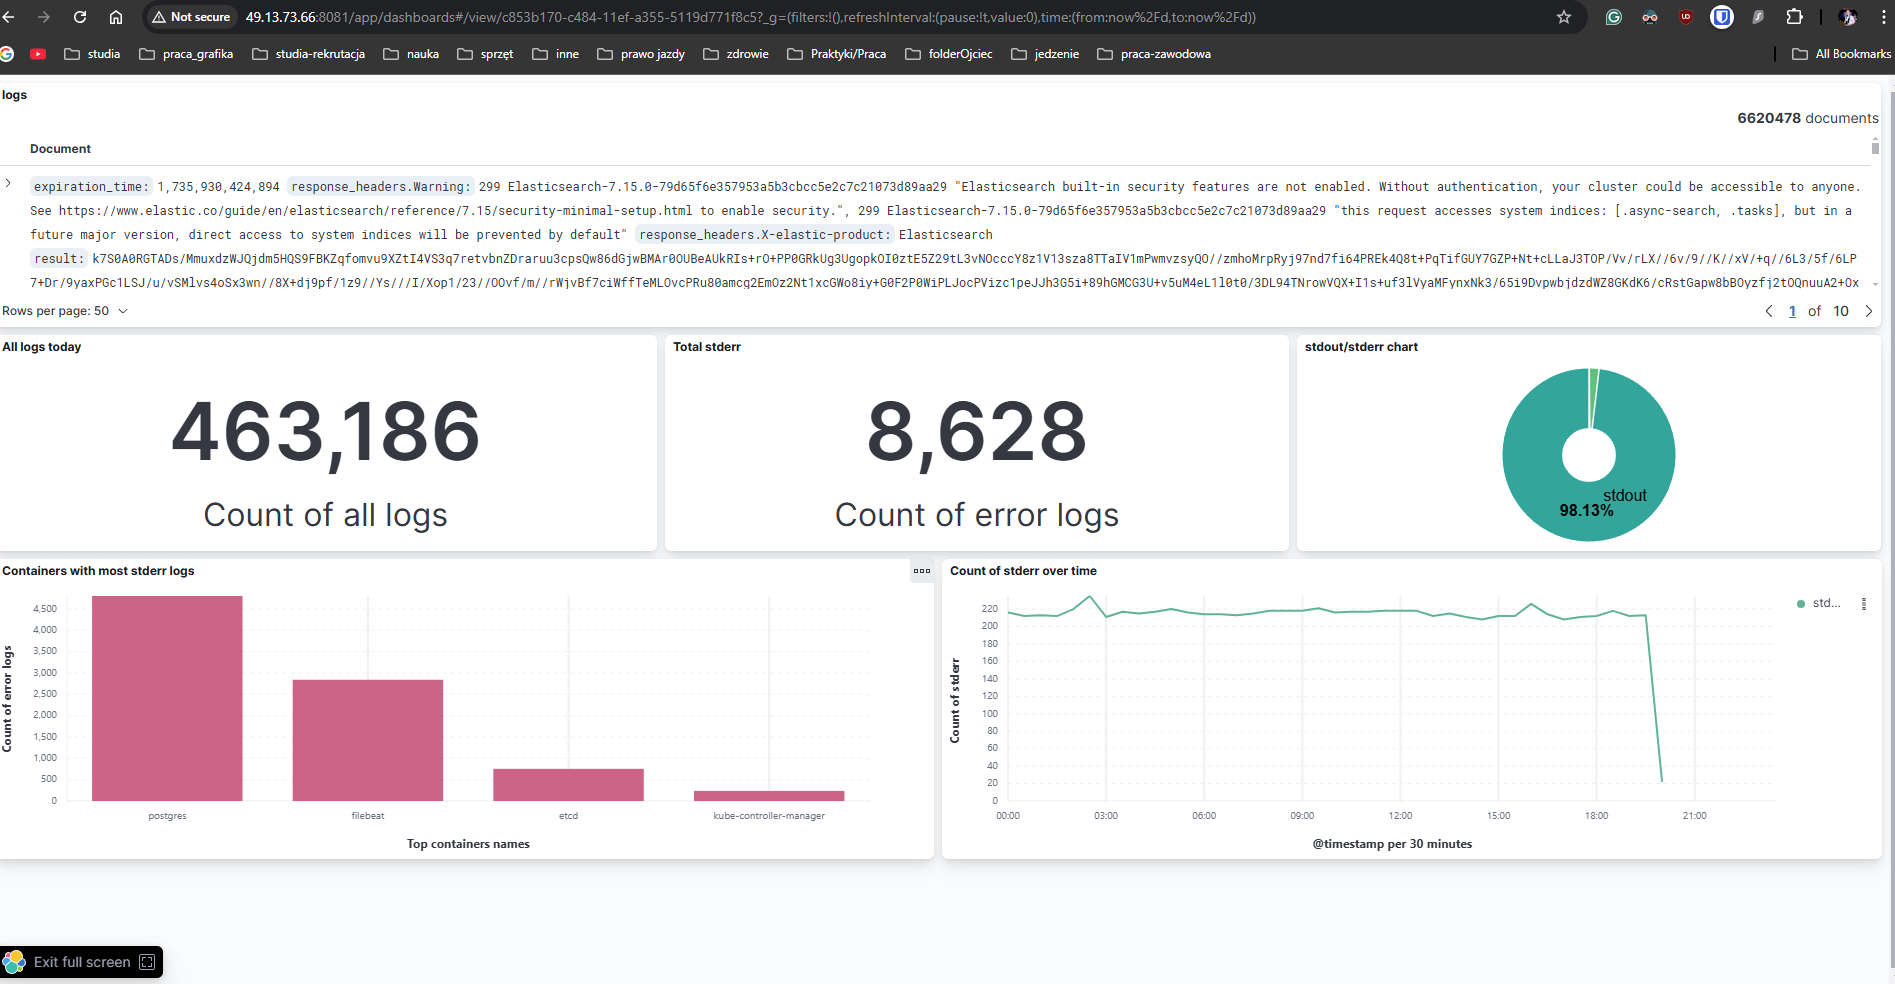
\includegraphics[width=1\linewidth]{img/monitor-dashboard.png}
    \caption{Wizualizacja podglądu logów}
    \label{fig:logs_dashboard}
\end{figure}
\input{tex/10-interfejs-użytkownika}
                            

%--------------------------------------------
% Literatura
%--------------------------------------------
\cleardoublepage % Zaczynamy od nieparzystej strony
\printbibliography

%--------------------------------------------
% Spisy (opcjonalne)
%--------------------------------------------
\newpage
\pagestyle{plain}

% Wykaz symboli i skrótów.
% Pamiętaj, żeby posortować symbole alfabetycznie
% we własnym zakresie. Ponieważ mało kto używa takiego wykazu,
% uznałem, że robienie automatycznie sortowanej listy
% na poziomie LaTeXa to za duży overkill.
% Makro \acronymlist generuje właściwy tytuł sekcji,
% w zależności od języka.
% Makro \acronym dodaje skrót/symbol do listy,
% zapewniając podstawowe formatowanie.
% //AB

\listoffigurestoc     % Spis rysunków.
\vspace{1cm}          % vertical space
\listoftablestoc      % Spis tabel.
\vspace{1cm}          % vertical space
\listofappendicestoc
W ramach pracy dołączono archiwum \texttt{kod.zip}, w którym znajdują się kod źródłowy podzielony na 3 foldery:
\begin{itemize}
   \item folder \texttt{back/} mający kod źródłowy aplikacji EMS-API,
   \item folder \texttt{front/} mający kod źródłowy interfejsu użytkownika,
   \item plik \texttt{dev-ops/} mający konfigurację środowiska wdrożeniowego.
\end{itemize}
Kod źródłowy dostępny jest również na publicznych github'ach:


\end{document} % Dobranoc.
